% Tom RYSER
% classe de document : article
% 
\documentclass[a4paper,12pt]{article}

% règles typographiques françaises
\usepackage[francais]{babel}
\usepackage[T1]{fontenc}
\usepackage[utf8]{inputenc}

% mise en page
\usepackage[left=3cm, right=3cm, top=1.5cm, bottom=1.5cm]{geometry}
\usepackage{fancyhdr}

%autre
\usepackage{hyperref}
\usepackage{graphicx}
\usepackage{listingsutf8}
\usepackage{xcolor}
\usepackage{fourier}
\usepackage{lastpage}
%titre
\title{modélisation du réseau TPG (2 lignes)}
\author{Tom RYSER}
\date{\today}

%cypherStyle
\definecolor{green}{HTML}{90a217}
\definecolor{string}{HTML}{c39f2f}
\definecolor{numbers}{HTML}{65bbb5}

\lstset{
	basicstyle=\normalfont\ttfamily,
	inputencoding=utf8/latin1, % needed for utf8 encoding
}

\lstdefinelanguage{Cypher}{
	basicstyle=\normalfont\ttfamily,
	breaklines=true,
	postbreak=\mbox{\textcolor{red}{$\hookrightarrow$}\space},
	keywords={create, match, detach, delete, set, where, and},
	keywordstyle=\color{green}\ttfamily,
	identifierstyle=\color{black},
	sensitive=false,
	comment=[l]{//},
	commentstyle=\color{gray}\ttfamily,
	stringstyle=\color{string}\ttfamily,
	morestring=[b]',
	morestring=[b]",
	numbers=left,
	numberstyle=\scriptsize,
	frame=single,
	extendedchars=true,
	literate=
	*{0}{{{\color{blue}0}}}1
	{1}{{{\color{blue}1}}}1
	{2}{{{\color{blue}2}}}1
	{3}{{{\color{blue}3}}}1
	{4}{{{\color{blue}4}}}1
	{5}{{{\color{blue}5}}}1
	{6}{{{\color{blue}6}}}1
	{7}{{{\color{blue}7}}}1
	{8}{{{\color{blue}8}}}1
	{9}{{{\color{blue}9}}}1
	{á}{{\'a}}1 {é}{{\'e}}1 {í}{{\'i}}1 {ó}{{\'o}}1 {ú}{{\'u}}1
	{Á}{{\'A}}1 {É}{{\'E}}1 {Í}{{\'I}}1 {Ó}{{\'O}}1 {Ú}{{\'U}}1
	{à}{{\`a}}1 {è}{{\`e}}1 {ì}{{\`i}}1 {ò}{{\`o}}1 {ù}{{\`u}}1
	{À}{{\`A}}1 {È}{{\'E}}1 {Ì}{{\`I}}1 {Ò}{{\`O}}1 {Ù}{{\`U}}1
	{ä}{{\"a}}1 {ë}{{\"e}}1 {ï}{{\"i}}1 {ö}{{\"o}}1 {ü}{{\"u}}1
	{Ä}{{\"A}}1 {Ë}{{\"E}}1 {Ï}{{\"I}}1 {Ö}{{\"O}}1 {Ü}{{\"U}}1
	{â}{{\^a}}1 {ê}{{\^e}}1 {î}{{\^i}}1 {ô}{{\^o}}1 {û}{{\^u}}1
	{Â}{{\^A}}1 {Ê}{{\^E}}1 {Î}{{\^I}}1 {Ô}{{\^O}}1 {Û}{{\^U}}1
	{Ã}{{\~A}}1 {ã}{{\~a}}1 {Õ}{{\~O}}1 {õ}{{\~o}}1
	{œ}{{\oe}}1 {Œ}{{\OE}}1 {æ}{{\ae}}1 {Æ}{{\AE}}1 {ß}{{\ss}}1
	{ű}{{\H{u}}}1 {Ű}{{\H{U}}}1 {ő}{{\H{o}}}1 {Ő}{{\H{O}}}1
	{ç}{{\c c}}1 {Ç}{{\c C}}1 {ø}{{\o}}1 {å}{{\r a}}1 {Å}{{\r A}}1
	{€}{{\euro}}1 {£}{{\pounds}}1 {«}{{\guillemotleft}}1
	{»}{{\guillemotright}}1 {ñ}{{\~n}}1 {Ñ}{{\~N}}1 {¿}{{?`}}1
}

\pagestyle{fancy}
\fancyhf{}
\fancyhead{}
\fancyfoot{}

\lhead{\author}
\rhead{\today}
\cfoot{\thepage\ sur \pageref{LastPage}}
%%%%%%%%%%%%%%%%%%% FIN DU PREAMBULE %%%%%%%%%%%%%%%%%%%%%%%%%%%%%%%%

\begin{document}

\begin{figure}
    \centering
    
\includegraphics[width=\linewidth]{img/logo.png}
    \maketitle
\end{figure}
\thispagestyle{empty}
  \clearpage 
\tableofcontents  \clearpage 
\section{Introduction}
Dans ce document je vais vous montré comment j'ai créer un graph neo4j pour obtenir des itinéraire des TPG
\section{insertion des données}
\danger tout les exemples proviennet de codes placé en annex.
\subsection{création des noeuds}
création de trois arrêt de bus avec leur nom et des coordonnée géographiques
\lstinputlisting[language=Cypher,caption=chemin le plus court entre 2 points, captionpos=b]{./listings/requeteCreateNode.cypher}

\begin{figure}[h]
    \centering
    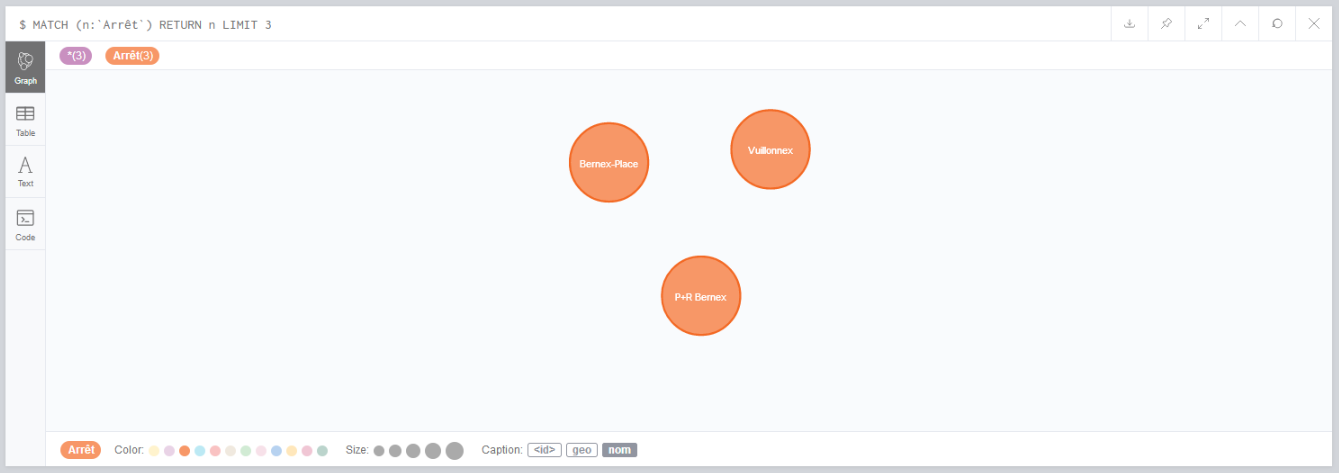
\includegraphics[width=\linewidth]{img/3nodes.png}
\end{figure}

\subsection{création des liaisons}
création des liaisons entre l'arrêt "P+R Bernex" et "Vuillonnex".
\lstinputlisting[language=Cypher,caption=chemin le plus court entre 2 points, captionpos=b]{./listings/requeteCreateLink.cypher}
\section{request}
    \subsection{chemin le plus court entre 2 points}
    \lstinputlisting[language=Cypher,caption=chemin le plus court entre 2 points, captionpos=b]{./listings/shortestPath.cypher}
\section{Problème encontré}
\paragraph{shortestPath}
\begin{itemize}
    \item Lors de la requête pour obtenir le chemin le plus cours entre 2 arrêts il m'est impossible de donner un sens à cette requête, les relations s'affichent dans les deux sens.
    \begin{itemize}
        \item Pour avoir un sens lors de l'affichage il faut mettre une flèche dans la requête " MATCH p = shortestPath((a)-[*]->(r)) " 
    \end{itemize}
    \item Après la mise à jour de neo4j à la version 3.5.3 du 7 Février, je n'ai plus pu utiliser l'application neo4j et j'ai passer la journée à essayer de la réparer.
    Le samedi 9 Février j'ai découvert Neo4j Sandbox qui permet de créer et intéragir avec un graph depuis une application web.

\end{itemize}
 
\section{Conclusion}
\section{Sources}
\lstinputlisting[language=Cypher,caption=fichier pour cr\'eer la base du graph, captionpos=b]{./listings/script_import.cypher}
\end{document}